\documentclass{article}
\usepackage{tikz}
\usepackage{rotating}
\usepackage{dirtree}
\usetikzlibrary{positioning, shapes}
\usepackage{hyperref}

\begin{document}

\begin{center}
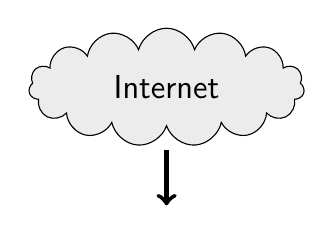
\begin{tikzpicture}[font=\large\sffamily, draw]
\node[cloud, cloud puffs=15, cloud ignores aspect, minimum width=3.5cm, minimum height=1.5cm, draw,fill=gray!15] (cloud) at (3, 0) {Internet};
\draw[ultra thick,->] (3, -0.8) -- (3, -1.5);
\end{tikzpicture}

% Overlay Parts (e.g VPC rectangle, Nginx -> NFS arrow)
\begin{tikzpicture}[font=\large\sffamily, overlay]
\node[rectangle, rounded corners, minimum width=13cm, minimum height=13cm, align=center, draw] at (0,-6.2) {};
\node[rectangle, rounded corners, minimum width=4.2cm, minimum height=2.1cm, align=center, draw=red,ultra thick,densely dashed] at (0,-7.05) {};
% Arrow from Nginx to NFS
\draw[ultra thick, purple,->] (-0.5, -0.95) -- (-4, -0.95) -- (-4, -10.5) -- (-1.4, -10.5);
\draw[ultra thick, dashed,->] (4, -0.95) -- (4, -10.5);
\node at (4.2, 0.55) {Virtual Private Cloud};
\node at (-4.2, 0.55) {Amazon Web Servic\begin{center}
    \begin{tikzpicture}[font=\large\sffamily, draw]
    \node[cloud, cloud puffs=15, cloud ignores aspect, minimum width=3.5cm, minimum height=1.5cm, draw,fill=gray!15] (cloud) at (3, 0) {Internet};
    \draw[ultra thick,->] (3, -0.8) -- (3, -1.5);
    \end{tikzpicture}
    
    % Overlay Parts (e.g VPC rectangle, Nginx -> NFS arrow)
    
\begin{tikzpicture}[font=\large\sffamily, overlay]
    \node[rectangle, rounded corners, minimum width=13cm, minimum height=13cm, align=center, draw] at (0,-6.2) {};
    \node[rectangle, rounded corners, minimum width=4.2cm, minimum height=2.1cm, align=center, draw=red,ultra thick,densely dashed] at (0,-7.05) {};
    % Arrow from Nginx to NFS
    \draw[ultra thick, purple,->] (-0.5, -0.95) -- (-4, -0.95) -- (-4, -10.5) -- (-1.4, -10.5);
    \draw[ultra thick, dashed,->] (4, -0.95) -- (4, -10.5);
    \node at (4.2, 0.55) {Virtual Private Cloud};
    \node at (-4.2, 0.55) {Amazon Web Services};
    \end{tikzpicture}
    
    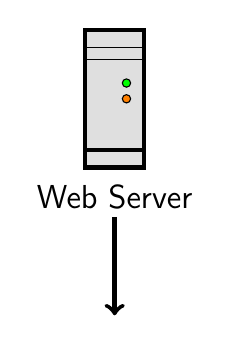
\begin{tikzpicture}[font=\large\sffamily,scale=1]
    \node[rectangle, minimum width=0.75cm, minimum height=1.75cm, align=center, draw,ultra thick,fill=gray!25] at (0,0) {}; 
    \draw (-0.35, 0.65) -- (0.35, 0.65);
    \draw (-0.35, 0.50) -- (0.35, 0.50);
    \draw[fill=green] (0.15,0.20) circle [radius=1.5pt];
    \draw[fill=orange] (0.15,0) circle [radius=1.5pt];
    \draw[ultra thick] (-0.35, -0.65) -- (0.35, -0.65);
    \node at (0, -1.25) {Web Server};
    \draw[ultra thick,->] (0, -1.5) -- (0, -2.75);
    \end{tikzpicture}
    
    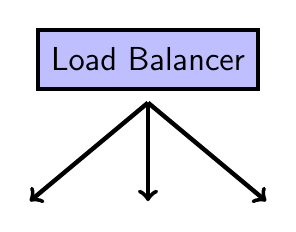
\begin{tikzpicture}[font=\large\sffamily]
    \node[rectangle, minimum width=2.8cm, minimum height=0.75cm, align=center, draw,ultra thick,fill=blue!25] at (0,0) {Load Balancer};
    \draw[ultra thick,->] (0, -0.55) -- (0, -1.8);
    \draw[ultra thick,->] (0, -0.55) -- (-1.5, -1.8);
    \draw[ultra thick,->] (0, -0.55) -- (1.5, -1.8);
    \end{tikzpicture}
    
    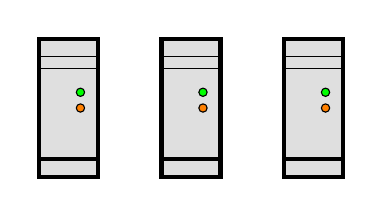
\begin{tikzpicture}[font=\large\sffamily]
        \tikzstyle{ann} = [draw=none,fill=none,right]
        \matrix[nodes={}, row sep=1.3cm,column sep=0.75cm, yshift=10cm] {
    \node[rectangle, minimum width=0.75cm, minimum height=1.75cm, align=center, draw,ultra thick,fill=gray!25] at (0,0) {}; 
    \draw (-0.35, 0.65) -- (0.35, 0.65);
    \draw (-0.35, 0.50) -- (0.35, 0.50);
    \draw[fill=green] (0.15,0.20) circle [radius=1.5pt];
    \draw[fill=orange] (0.15,0) circle [radius=1.5pt];
    \draw[ultra thick] (-0.35, -0.65) -- (0.35, -0.65); &
    
    \node[rectangle, minimum width=0.75cm, minimum height=1.75cm, align=center, draw,ultra thick,fill=gray!25] at (0,0) {}; 
    \draw (-0.35, 0.65) -- (0.35, 0.65);
    \draw (-0.35, 0.50) -- (0.35, 0.50);
    \draw[fill=green] (0.15,0.20) circle [radius=1.5pt];
    \draw[fill=orange] (0.15,0) circle [radius=1.5pt];
    \draw[ultra thick] (-0.35, -0.65) -- (0.35, -0.65); &
    
    \node[rectangle, minimum width=0.75cm, minimum height=1.75cm, align=center, draw,ultra thick,fill=gray!25] at (0,0) {}; 
    \draw (-0.35, 0.65) -- (0.35, 0.65);
    \draw (-0.35, 0.50) -- (0.35, 0.50);
    \draw[fill=green] (0.15,0.20) circle [radius=1.5pt];
    \draw[fill=orange] (0.15,0) circle [radius=1.5pt];
    \draw[ultra thick] (-0.35, -0.65) -- (0.35, -0.65);\\
        };
    \end{tikzpicture}
    
    
\begin{tikzpicture}[font=\large\sffamily,scale=1]
    \node at (0, -3.8) {Auto-scaled PHP-FPM instances};
    \draw[ultra thick,->] (0, -4.0) -- (-1, -4.8);
    \draw[ultra thick,->] (0, -4.0) -- (1, -4.8);
    \end{tikzpicture}
    
    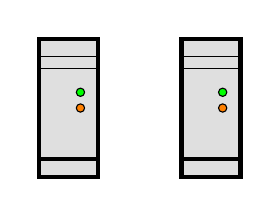
\begin{tikzpicture}[font=\large\sffamily]
        \matrix[nodes={draw, ultra thick, fill=blue!20}, row sep=1.3cm,column sep=1cm, yshift=5cm] {
    \node[rectangle, minimum width=0.75cm, minimum height=1.75cm, align=center, draw,ultra thick,fill=gray!25] at (0,0) {}; 
    \draw (-0.35, 0.65) -- (0.35, 0.65);
    \draw (-0.35, 0.50) -- (0.35, 0.50);
    \draw[fill=green] (0.15,0.20) circle [radius=1.5pt];
    \draw[fill=orange] (0.15,0) circle [radius=1.5pt];
    \draw[ultra thick] (-0.35, -0.65) -- (0.35, -0.65);&
    
    \node[rectangle, minimum width=0.75cm, minimum height=1.75cm, align=center, draw,ultra thick,fill=gray!25] at (0,0) {}; 
    \draw (-0.35, 0.65) -- (0.35, 0.65);
    \draw (-0.35, 0.50) -- (0.35, 0.50);
    \draw[fill=green] (0.15,0.20) circle [radius=1.5pt];
    \draw[fill=orange] (0.15,0) circle [radius=1.5pt];
    \draw[ultra thick] (-0.35, -0.65) -- (0.35, -0.65);\\
        };
    \end{tikzpicture}
    
    \begin{tikzpicture}[font=\large\sffamily,overlay]
    \node at (-2.15, 0.1) {Network File Server};
    \node at (1.875, 0.1) {Database Server};
    \begin{sideways}
    \node[blue] at (6, 4.275) {Static File Requests};
    \begin{turn}{-180}
    \node at (-6, 4.275) {Internal Requests Over Private IP Address};
    \end{turn}
    \end{sideways}
    \end{tikzpicture}
    
    \end{center}es};
\end{tikzpicture}

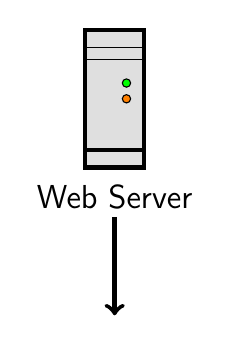
\begin{tikzpicture}[font=\large\sffamily,scale=1]
\node[rectangle, minimum width=0.75cm, minimum height=1.75cm, align=center, draw,ultra thick,fill=gray!25] at (0,0) {}; 
\draw (-0.35, 0.65) -- (0.35, 0.65);
\draw (-0.35, 0.50) -- (0.35, 0.50);
\draw[fill=green] (0.15,0.20) circle [radius=1.5pt];
\draw[fill=orange] (0.15,0) circle [radius=1.5pt];
\draw[ultra thick] (-0.35, -0.65) -- (0.35, -0.65);
\node at (0, -1.25) {Web Server};
\draw[ultra thick,->] (0, -1.5) -- (0, -2.75);
\end{tikzpicture}

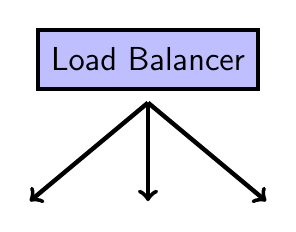
\begin{tikzpicture}[font=\large\sffamily]
\node[rectangle, minimum width=2.8cm, minimum height=0.75cm, align=center, draw,ultra thick,fill=blue!25] at (0,0) {Load Balancer};
\draw[ultra thick,->] (0, -0.55) -- (0, -1.8);
\draw[ultra thick,->] (0, -0.55) -- (-1.5, -1.8);
\draw[ultra thick,->] (0, -0.55) -- (1.5, -1.8);
\end{tikzpicture}

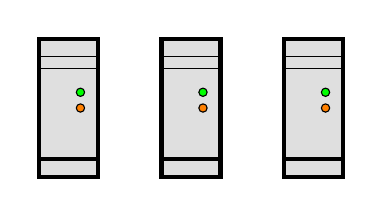
\begin{tikzpicture}[font=\large\sffamily]
    \tikzstyle{ann} = [draw=none,fill=none,right]
    \matrix[nodes={}, row sep=1.3cm,column sep=0.75cm, yshift=10cm] {
\node[rectangle, minimum width=0.75cm, minimum height=1.75cm, align=center, draw,ultra thick,fill=gray!25] at (0,0) {}; 
\draw (-0.35, 0.65) -- (0.35, 0.65);
\draw (-0.35, 0.50) -- (0.35, 0.50);
\draw[fill=green] (0.15,0.20) circle [radius=1.5pt];
\draw[fill=orange] (0.15,0) circle [radius=1.5pt];
\draw[ultra thick] (-0.35, -0.65) -- (0.35, -0.65); &

\node[rectangle, minimum width=0.75cm, minimum height=1.75cm, align=center, draw,ultra thick,fill=gray!25] at (0,0) {}; 
\draw (-0.35, 0.65) -- (0.35, 0.65);
\draw (-0.35, 0.50) -- (0.35, 0.50);
\draw[fill=green] (0.15,0.20) circle [radius=1.5pt];
\draw[fill=orange] (0.15,0) circle [radius=1.5pt];
\draw[ultra thick] (-0.35, -0.65) -- (0.35, -0.65); &

\node[rectangle, minimum width=0.75cm, minimum height=1.75cm, align=center, draw,ultra thick,fill=gray!25] at (0,0) {}; 
\draw (-0.35, 0.65) -- (0.35, 0.65);
\draw (-0.35, 0.50) -- (0.35, 0.50);
\draw[fill=green] (0.15,0.20) circle [radius=1.5pt];
\draw[fill=orange] (0.15,0) circle [radius=1.5pt];
\draw[ultra thick] (-0.35, -0.65) -- (0.35, -0.65);\\
    };
\end{tikzpicture}


\begin{tikzpicture}[font=\large\sffamily,scale=1]
\node at (0, -3.8) {Auto-scaled PHP-FPM instances};
\draw[ultra thick,->] (0, -4.0) -- (-1, -4.8);
\draw[ultra thick,->] (0, -4.0) -- (1, -4.8);
\end{tikzpicture}

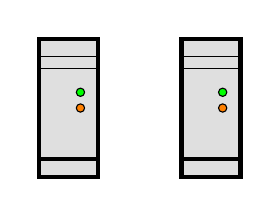
\begin{tikzpicture}[font=\large\sffamily]
    \matrix[nodes={draw, ultra thick, fill=blue!20}, row sep=1.3cm,column sep=1cm, yshift=5cm] {
\node[rectangle, minimum width=0.75cm, minimum height=1.75cm, align=center, draw,ultra thick,fill=gray!25] at (0,0) {}; 
\draw (-0.35, 0.65) -- (0.35, 0.65);
\draw (-0.35, 0.50) -- (0.35, 0.50);
\draw[fill=green] (0.15,0.20) circle [radius=1.5pt];
\draw[fill=orange] (0.15,0) circle [radius=1.5pt];
\draw[ultra thick] (-0.35, -0.65) -- (0.35, -0.65);&

\node[rectangle, minimum width=0.75cm, minimum height=1.75cm, align=center, draw,ultra thick,fill=gray!25] at (0,0) {}; 
\draw (-0.35, 0.65) -- (0.35, 0.65);
\draw (-0.35, 0.50) -- (0.35, 0.50);
\draw[fill=green] (0.15,0.20) circle [radius=1.5pt];
\draw[fill=orange] (0.15,0) circle [radius=1.5pt];
\draw[ultra thick] (-0.35, -0.65) -- (0.35, -0.65);\\
    };
\end{tikzpicture}

\begin{tikzpicture}[font=\large\sffamily,overlay]
\node at (-2.15, 0.1) {Network File Server};
\node at (1.875, 0.1) {Database Server};
\begin{sideways}
\node[blue] at (6, 4.275) {Static File Requests};
\begin{turn}{-180}
\node at (-6, 4.275) {Internal Requests Over Private IP Address};
\end{turn}
\end{sideways}
\end{tikzpicture}

\end{center}
\end{document}